\section{Performance}
\todo[inline]{
- is the effect size valuable?

- Cohen’s effect size value (d = .62) suggested a moderate to high practical significance.

- comparison to other predictor displays

- Keystrokes per exp

- Learning effects

- Computer and gaming frequency

- can the data be misinterpreted?

- what could be done differently?

- this is a test on how it works on intuition, they may have performed better if they were told how the PD works
}

\missingfigure{Table with the performance in comparison with other displays}

\missingfigure{Graph showing number of keystrokes for each experiment}

\missingfigure{Learning effect for each display}

\missingfigure{Gamers vs non gamers}

In addition, \figref{score_key_relationship_2} shows a scatter plot of score and number of key presses for the no delay condition. It shows a moderate positive linear relationship 

\begin{figure}[h!]
    \centering
    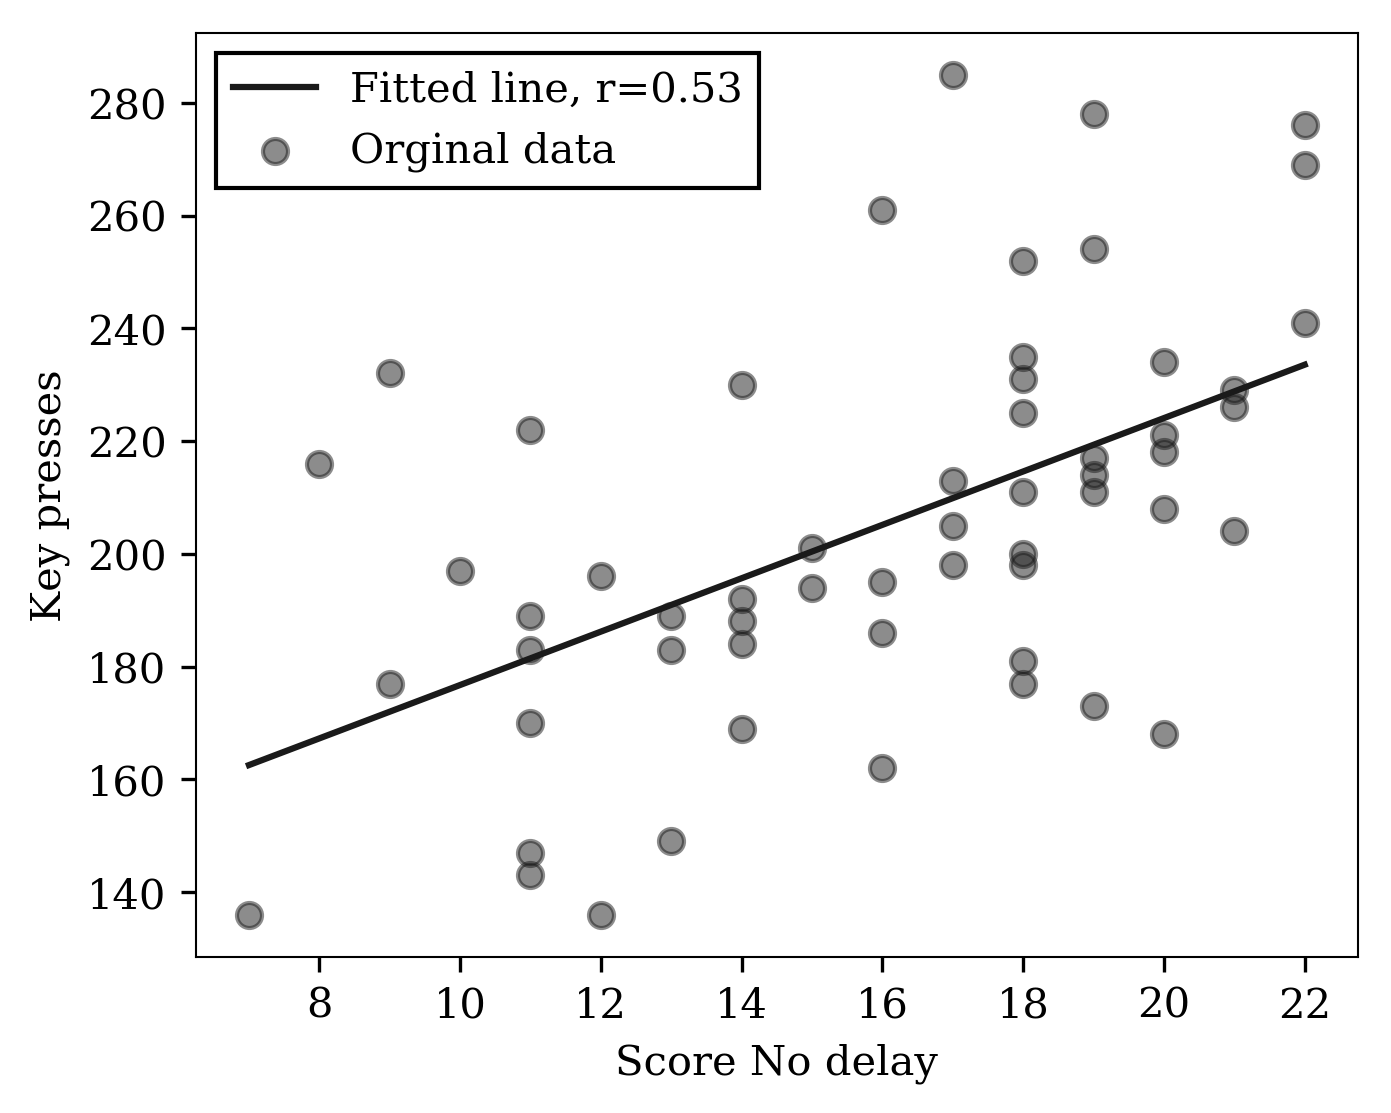
\includegraphics[scale=0.85]{score_key_relationship_2}
    \caption{Score and number of key presses correlation for the no delay display.}
    \label{score_key_relationship_2}
\end{figure}

\section{Subjective measurements}
\todo[inline]{
- discussion on TLX

- Subjective delay times

- Subjective performance vs real performance
}

\missingfigure{Subjective performance vs real performance}

\section{Hypothesis}
\todo[inline]{
MOVE TO DISCUSSION
}
\todo[inline]{
- Hypothesis

- novelty of solution
}

\section{Future work}
\subsection{Predictive display}
\todo[inline]{
- h264 compression tracking could be used for live improvement of the predictor display

- it might be better to crop with different windows instead of moving the video, people reported that it was disturbing

- many get fixated on the real center pin even though there is a red arrow there, it would be interesting to see if they performed better without any real reference

- wider FOV

- live machine learning to better predict the movement (speed, incline, battery power etc.)
}
\subsection{eduROV package}
\todo[inline]{
- websockets

- flask?
}